\documentclass[final]{statsoc}
\pdfoutput=1    % Make Arxiv happy

\RequirePackage[a4paper]{geometry}
\RequirePackage[OT1]{fontenc}
\RequirePackage{graphicx}
\RequirePackage{enumerate}
\RequirePackage{booktabs}
\RequirePackage{color, colortbl, transparent}
\RequirePackage{multirow}
\RequirePackage{amssymb}
\RequirePackage[cmex10]{amsmath}
\RequirePackage{placeins}
\RequirePackage{xtab}

\RequirePackage[caption=false]{subfig}


%\startlocaldefs

% The below are from iproc.aux, to match equation/figure/section numbers
\newlabel{T:mple-approx-error}{{4.2}{8}}
\newlabel{E:log-pl-multiple-approx}{{8}{7}}
\newlabel{E:cox-intensity}{{1}{3}}
\newlabel{T:group-dynamic}{{6}{16}}
\newlabel{S:enron-covariates}{{5.2}{10}}
\newlabel{F:enron-net-indicator}{{7}{17}}

\definecolor{Gray}{gray}{0.9}
\definecolor{LightGray}{gray}{0.5}

\usepackage{iproc-macros}
\newcommand{\qedhere}{}
%\endlocaldefs

\title[Point Process Modeling for Directed Interaction Networks: Supplementary Material]{%
    Point process modeling for directed interaction networks: Supplementary material
}

\author[P.\ O.\ Perry]{%
    Patrick O.\ Perry
}

\address{Stern School of Business, New York University, USA}

\author[P.\ J.\ Wolfe]{%
    Patrick J.\ Wolfe
}

\address{Department of Statistical Science, University College London, UK}

\received{November 2010}
\revised{October 2012}

\runauthor{%
    P.\ O.\ Perry and P.\ J.\ Wolfe
}

\coaddress{
Patrick O.\ Perry,
Information, Operations, and Management Sciences Department,
Stern School of Business,
New York University,
44 West 4th St,
New York, NY 10012,~USA
}
\email{pperry@stern.nyu.edu}


\begin{document}


\section{Simulation study}

We show a simulation study to empirically verify the result of
Theorem~\ref{T:mple-approx-error} from the main text.  In the study, we have one sender,
and a receiver count $|\mathcal{J}|$ ranging from $32$ to $1000$.  Each
receiver was assigned a constant coefficient vector $x(j)$ whose elements were
independent Bernoulli random variables with success probability $\tfrac{1}{2}$.
The components of the true coefficient vector $\beta$ were drawn independently
from the standard normal distribution.

We chose sample sizes $n$ ranging from 32 to 100,000.  For each receiver count
$|\mathcal{J}|$, we drew $n$ multicast messages, with the receiver set $J_m$ for
message $m$ determined as follows:
we determined the size, $|J_m|$, by drawing from a geometric distribution
with success probability $p = 0.4$, so that $\mathbb{P}\{|J_m| = L\} = (1 - p)^{L -
1} \, p$ for $L \geq 1$; once $|J_m|$ was determined, we chose among
all receiver sets with cardinality $|J_m|$, with
$\mathbb{P}\{ J_m = J \} \propto \exp\{ \sum_{j \in J} \beta^\trans x(j)\}$.
Once we generated the message data, we computed $\tilde \beta$ by maximizing
the approximate log partial likelihood analogous
to~\eqref{E:log-pl-multiple-approx} from the main text.  Finally, we computed $\|\beta - \tilde
\beta\|$.

We repeated this procedure for 100 random replicates at each receiver count
and sample size, and computed the mean squared error of $\tilde \beta$ by
averaging the value of $\|\beta - \tilde \beta\|^2$ over all replicates.
Figure~\ref{F:multicast-error} overleaf displays the results.  From the spacings of the
asymptotes of the solid lines in the figure, we can see that if
$|\mathcal{J}|$ does not grow with $n$, then the error $\|\beta - \tilde
\beta\|^2$ is roughly $\Oh(|\mathcal{J}|^{-2})$ for large $n$; strictly
speaking, the assumptions of Theorem~\ref{T:mple-approx-error} from the main text do not hold in
this scenario since $G_n = \OhP(n / |\mathcal{J}|)$, but nevertheless the
theorem predicts an error rate of $\Oh(|\mathcal{J}|^{-2})$.  For
Theorem~\ref{T:mple-approx-error} from the main text to apply, we require that $|\mathcal{J}|$
grow with $n$.  From the slope of the dashed line in
Fig.~\ref{F:multicast-error} overleaf, we can see that if $|\mathcal{J}| = \sqrt{n}$,
then $\|\beta - \tilde \beta\|^2$ is roughly $\OhP(n^{-1})$; this agrees with
the theorem, since $G_n = \sqrt{n}$ in this situation.



\begin{figure}[!t]
  \centering
  \makebox{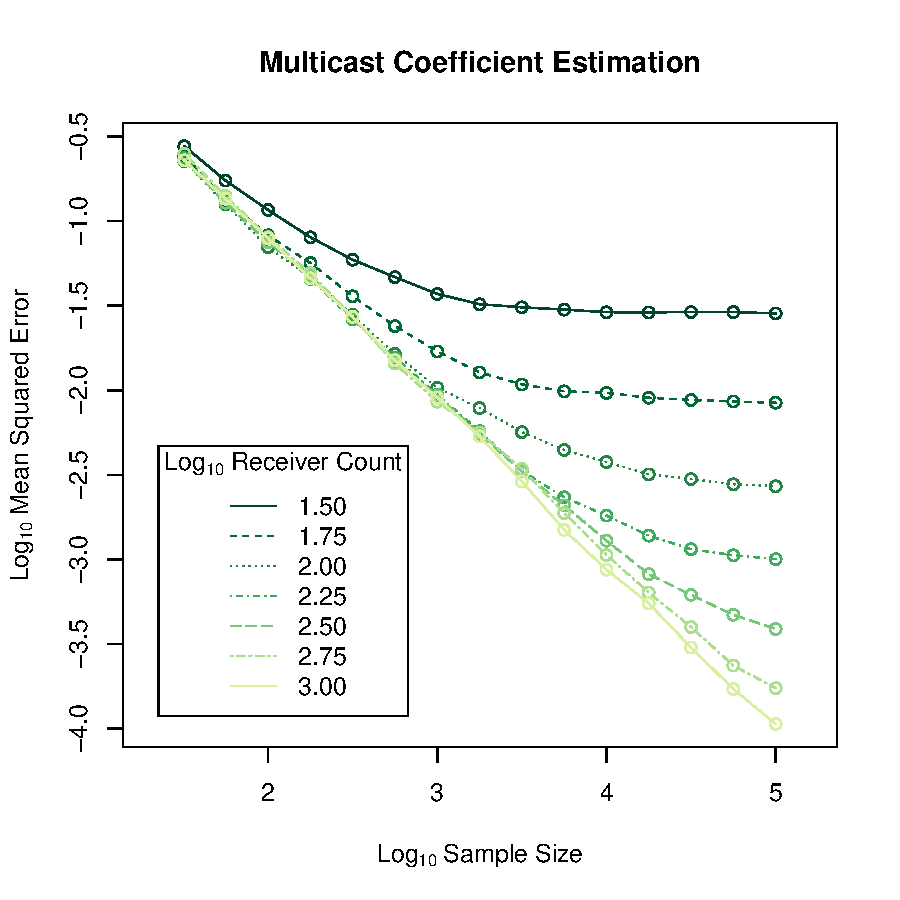
\includegraphics[scale=0.6]{figures/multicast-error}}
  \caption{
	\captiontitle{Multicast coefficient estimation error with approximate MPLE}
	Receiver count~$|\mathcal{J}|$ is equal to the square root of sample size~$n$
	along the dashed line.
  }\label{F:multicast-error}
\end{figure}



\section{Comparative analyses}\label{S:comparative}

\subsection{A comparative analysis based on contingency tables}
\label{sec:contin-analysis}

Were we interested only in homophily, we might be tempted to forgo
the proportional intensity model of~\eqref{E:cox-intensity} from the main text, and instead
perform a contingency table analysis.  However, as we now describe,
such an analysis leads to very different conclusions
about the predictive strength of homophily in our data.

For example, suppose that we are interested in testing for seniority-based homophily.  Ignoring
network effects and other dependency, we might model $\Prob\{ i \to j \mid i
\}$, the probability of employee $j$ being the recipient of a message given
that employee $i$ is the sender, by way of a multinomial logit model:
\[
  \Prob\{ i \to j \mid i \}
    \propto \exp\{ \beta_J J(j) + \beta_{JJ} J(i) J(j) \}.
\]
In this setting,
Junior-Junior homophily would manifest in a positive value of
$\beta_{J} + \beta_{JJ}$ and Senior-Senior homophily would manifest in
a negative value of $\beta_J$.

Since there are $n_J = 82$ Junior
executives and $n_S = 74$ Senior executives, and since the sender and
receiver of a message are distinct, we have that
\begin{align*}
  \Prob\{ i \to j \mid i, J(i) = 1 \}
    &=
      \frac{e^{(\beta_J + \beta_{JJ}) J(j)}}
           {(n_J - 1) e^{\beta_J + \beta_{JJ}} + n_S} \\
  \Prob\{ i \to j \mid i, J(i) = 0 \},
    &=
      \frac{e^{\beta_J J(j)}}
           {n_J e^{\beta_J} + (n_S - 1)}.
\end{align*}
In turn, we compute the corresponding maximum likelihood coefficient estimates using the
entries of a $2 \times 2$ table that counts the number of messages exchanged
between each group:
\begin{center}
\begin{tabular}{lrr}
  \toprule
  & \multicolumn{2}{c}{Receiver} \\
  \cmidrule(l){2-3}
  Sender & Junior & Senior \\
  \midrule
  Junior &  7972  &  5833 \\
  Senior &  3977  & 14479 \\
  \bottomrule
\end{tabular}
\end{center}
The resultant estimates are $\hat \beta_{J} = -1.4$ and
$\hat \beta_{JJ} = 1.6$, with (Wald) standard errors of about $0.02$
for each.  Indeed, these are exactly the estimated coefficients we would
obtain if we were to use the proportional intensity model
$\lambda_t(i,j) = \bar \lambda_t(i) \exp\{ \beta_J J(j) + \beta_{JJ} J(i) J(j)
\}$, a result that holds more generally for non-time-varying covariates.

One problem with this analysis is that we have marginalized over the
other covariates (Gender and Department), potentially introducing a Simpson's
paradox.  This issue is easily rectified, however, by introducing covariates for senders and
receivers, along with the corresponding second-order covariate interactions;
Fig.~\ref{T:group-static} above shows the resulting coefficient estimates.

\begin{figure}
  \centering
  \makebox[\textwidth]{
    \scriptsize
    \begin{tabular}{lrrrrrrrrrr}
\toprule
& \multicolumn{10}{c}{Receiver} \\
\cmidrule(l){2-11} 
Sender & \multicolumn{1}{c}{1} & \multicolumn{1}{c}{L} & \multicolumn{1}{c}{T} & \multicolumn{1}{c}{J} & \multicolumn{1}{c}{F} & \multicolumn{1}{c}{LJ} & \multicolumn{1}{c}{TJ} & \multicolumn{1}{c}{LF} & \multicolumn{1}{c}{TF} & \multicolumn{1}{c}{JF} \\
\midrule
\multirow{2}{*}{L} &-0.22 &\cellcolor{Gray}1.96 &\textcolor{LightGray}{-0.03} &-1.87 &-0.67 &0.85 &2.64 &2.02 &\textcolor{LightGray}{1.08} &0.82\\
 &\tiny{(0.05)} &\cellcolor{Gray}\tiny{(0.06)} &\textcolor{LightGray}{\tiny{(0.11)}} &\tiny{(0.22)} &\tiny{(0.09)} &\tiny{(0.21)} &\tiny{(0.30)} &\tiny{(0.13)} &\textcolor{LightGray}{\tiny{(0.41)}} &\tiny{(0.15)}\\[1ex]
\multirow{2}{*}{T} &-1.95 &-0.59 &\cellcolor{Gray}2.58 &2.76 &-0.45 &\textcolor{LightGray}{0.20} &-1.72 &1.05 &3.19 &-1.65\\
 &\tiny{(0.06)} &\tiny{(0.09)} &\cellcolor{Gray}\tiny{(0.08)} &\tiny{(0.10)} &\tiny{(0.10)} &\textcolor{LightGray}{\tiny{(0.15)}} &\tiny{(0.18)} &\tiny{(0.16)} &\tiny{(0.32)} &\tiny{(0.13)}\\[1ex]
\multirow{2}{*}{J} &-3.21 &-2.49 &2.56 &\cellcolor{Gray}4.26 &\textcolor{LightGray}{0.19} &-1.47 &-1.70 &1.95 &2.26 &-1.65\\
 &\tiny{(0.09)} &\tiny{(0.19)} &\tiny{(0.11)} &\cellcolor{Gray}\tiny{(0.12)} &\textcolor{LightGray}{\tiny{(0.12)}} &\tiny{(0.24)} &\tiny{(0.19)} &\tiny{(0.23)} &\tiny{(0.32)} &\tiny{(0.15)}\\[1ex]
\multirow{2}{*}{F} &\textcolor{LightGray}{-0.09} &-0.62 &\textcolor{LightGray}{-0.16} &\textcolor{LightGray}{0.14} &\cellcolor{Gray}0.71 &0.86 &-3.85 &\textcolor{LightGray}{-0.14} &\textcolor{LightGray}{0.83} &\textcolor{LightGray}{-0.36}\\
 &\textcolor{LightGray}{\tiny{(0.05)}} &\tiny{(0.08)} &\textcolor{LightGray}{\tiny{(0.10)}} &\textcolor{LightGray}{\tiny{(0.12)}} &\cellcolor{Gray}\tiny{(0.07)} &\tiny{(0.17)} &\tiny{(0.28)} &\textcolor{LightGray}{\tiny{(0.17)}} &\textcolor{LightGray}{\tiny{(0.31)}} &\textcolor{LightGray}{\tiny{(0.14)}}\\[1ex]
\multirow{2}{*}{LJ} &1.53 &1.18 &\textcolor{LightGray}{0.01} &-1.35 &\textcolor{LightGray}{0.15} &\cellcolor{Gray}\textcolor{LightGray}{0.76} &-3.03 &-1.68 &\textcolor{LightGray}{0.56} &0.98\\
 &\tiny{(0.16)} &\tiny{(0.22)} &\textcolor{LightGray}{\tiny{(0.21)}} &\tiny{(0.32)} &\textcolor{LightGray}{\tiny{(0.23)}} &\cellcolor{Gray}\textcolor{LightGray}{\tiny{(0.36)}} &\tiny{(0.41)} &\tiny{(0.30)} &\textcolor{LightGray}{\tiny{(0.49)}} &\tiny{(0.21)}\\[1ex]
\multirow{2}{*}{TJ} &1.43 &4.29 &-1.65 &-2.00 &-1.53 &-2.15 &\cellcolor{Gray}\textcolor{LightGray}{0.40} &\textcolor{LightGray}{0.68} &\textcolor{LightGray}{-1.21} &1.15\\
 &\tiny{(0.18)} &\tiny{(0.26)} &\tiny{(0.20)} &\tiny{(0.20)} &\tiny{(0.24)} &\tiny{(0.32)} &\cellcolor{Gray}\textcolor{LightGray}{\tiny{(0.26)}} &\textcolor{LightGray}{\tiny{(0.32)}} &\textcolor{LightGray}{\tiny{(0.37)}} &\tiny{(0.22)}\\[1ex]
\multirow{2}{*}{LF} &-2.82 &2.13 &\textcolor{LightGray}{0.50} &\textcolor{LightGray}{0.66} &\textcolor{LightGray}{0.70} &\textcolor{LightGray}{-0.55} &5.29 &\cellcolor{Gray}\textcolor{LightGray}{-0.04} &-2.48 &\textcolor{LightGray}{-0.59}\\
 &\tiny{(0.18)} &\tiny{(0.19)} &\textcolor{LightGray}{\tiny{(0.25)}} &\textcolor{LightGray}{\tiny{(0.34)}} &\textcolor{LightGray}{\tiny{(0.25)}} &\textcolor{LightGray}{\tiny{(0.35)}} &\tiny{(0.45)} &\cellcolor{Gray}\textcolor{LightGray}{\tiny{(0.29)}} &\tiny{(0.40)} &\textcolor{LightGray}{\tiny{(0.20)}}\\[1ex]
\multirow{2}{*}{TF} &-2.57 &\textcolor{LightGray}{-0.09} &2.83 &2.15 &0.99 &\textcolor{LightGray}{-0.17} &1.40 &\textcolor{LightGray}{-0.94} &\cellcolor{Gray}-2.41 &\textcolor{LightGray}{-0.25}\\
 &\tiny{(0.28)} &\textcolor{LightGray}{\tiny{(0.36)}} &\tiny{(0.29)} &\tiny{(0.29)} &\tiny{(0.27)} &\textcolor{LightGray}{\tiny{(0.39)}} &\tiny{(0.36)} &\textcolor{LightGray}{\tiny{(0.29)}} &\cellcolor{Gray}\tiny{(0.33)} &\textcolor{LightGray}{\tiny{(0.26)}}\\[1ex]
\multirow{2}{*}{JF} &1.88 &0.91 &-1.38 &-1.46 &-0.53 &\textcolor{LightGray}{0.30} &2.09 &\textcolor{LightGray}{-0.04} &\textcolor{LightGray}{0.13} &\cellcolor{Gray}\textcolor{LightGray}{0.54}\\
 &\tiny{(0.11)} &\tiny{(0.15)} &\tiny{(0.14)} &\tiny{(0.15)} &\tiny{(0.14)} &\textcolor{LightGray}{\tiny{(0.20)}} &\tiny{(0.21)} &\textcolor{LightGray}{\tiny{(0.19)}} &\textcolor{LightGray}{\tiny{(0.29)}} &\cellcolor{Gray}\textcolor{LightGray}{\tiny{(0.17)}}\\[1ex]
\bottomrule
\end{tabular}

  }
  \caption{
    Estimated coefficients and standard errors for the contingency table-based analysis of Section~\ref{sec:contin-analysis}
  }
  \label{T:group-static}
\end{figure}

The far more important
problem is that this analysis implicitly assumes each message to be
independent and identically distributed, conditional on the sender of
the message.  This assumption is blatantly false: common sense tells us that if Junior $A$ sends a message
to Junior $B$, then the next time $B$ sends a message, $B$ is more likely to
choose $A$ as a recipient.  Any homophily effect present in these interaction
data is thus likely to be exaggerated by reciprocation and other network effects.  Indeed,
comparing the contingency table-based estimates in Fig.~\ref{T:group-static} above
with the estimates from the proportional intensity model with network effects
in Fig.~\ref{T:group-dynamic} from the main text, we can see that the coefficient estimates are
much higher when we don't adjust for network effects.  Thus even in cases where network effects themselves
are not the object of primary interest, it is important to account for them when
making inferences about the predictive strength of other covariates.


\subsection{Comparative analyses using actor-oriented and exponential random graph models}
\label{S:actor-ergm-comparison}

A number of dynamic network models exist in the literature, including
\citefullauthor{hanneke2010discrete}'s~(\citeyear{hanneke2010discrete})
exponential random graph model with time-varying coefficients,  and
\citefullauthor{kolar2010estimating}'s~(\citeyear{kolar2010estimating})
time-varying stochastic block model.  Alternative approaches explicitly based
on point processes, but excluding network effects and other covariate
information, include that of \citet{malmgen2009characterizing}, who model
activity at the level of the individual using a hidden Markov model, and of
\citet{heard2010bayesian}, who work at the level of the dyad, assuming a
piecewise-constant interaction rate.  The closest match to our approach is
given by the actor-oriented model of
\citet{snijders2001statistical,snijders2005models}, which we now detail in
Section~\ref{sec:actor-oriented} below.
Then, in Section~\ref{S:ERGM}, we provide a comparison to a static network
analysis based on an exponential random graph model.

\subsubsection{Actor-oriented model analysis}\label{sec:actor-oriented}

The actor-oriented model is designed for a sequence of snapshots $G_1$,
$G_2,\dotsc,$ of network activity, where each $G_t$ is an $I \times J$ binary
matrix representing pairwise connectivity between actors at time~$t$.  The
model is best suited for ties that persist in time, not instantaneous events;
it treats the sequence of networks as a first-order Markov chain, with the
distribution of $G_t$ determined by $G_{t-1}$.  Actors are assumed to change
their ties between times $t-1$ and $t$ to maximize a stochastic utility
function that depends on characteristics of the overall network.  Essentially,
given that the network is in state $G$, and that actor $i$ is allowed to make
a change, he will change his link to actor $j$ according to
\[
  p(j | i, G) \propto
    \exp\Big\{ \sum_{s=1}^S \beta_s T_s\big(G(i \leadsto j)\big)
      +
        \sum_{s=1}^{S'} \beta'_s T'_s(G \setminus \{ i \to j\})
    \Big\},
\]
where $T_s$ and $T'_s$ are network statistics; $\beta_s$ and $\beta_s'$ are
unknown coefficients; $G(i \leadsto j)$ denotes the network obtained either by
adding link $i \to j$ if it is absent or removing link $i \to j$ if it is
present; $G \setminus \{ i \to j \}$ denotes the network obtained by removing
$i \to j$ if it is present.  Additionally, the rate at which actor $i$ changes
ties between observation times $t-1$ and $t$ is given by $\lambda(i)$,
specified via another parametric model.  (See \citet{snijders2010introduction}
for a more thorough introduction.)  The change probability function $p(j | i,
G)$ plays a similar role to the multiplier $\exp\{ x_t(i,j)^\trans \beta \}$
in the proportional intensity model from the main text, and the change rate function $\lambda(i)$
plays a similar role to the baseline intensity $\bar \lambda_t(i)$.

For purposes of comparison, we specified a change probability model $p(j | i,
G)$ with network statistics analogous to those used in
Section~\ref{S:enron-covariates} from the main text, and then we estimated coefficient sets
$\beta$ and $\beta'$ analogous to the coefficients in the proportional intensity
model.  We used the \texttt{RSiena} package \citep{rsiena2011} to specify and
fit the actor-oriented model after binning the Enron e-mail interaction data
at regular intervals to obtain network snapshots $G_1$, $G_2$, and $G_3$.
Here, $G_t(i,j) = 1$ if message $i \to j$ was observed in period $t$, and
$G_t(i,j) = 0$ otherwise; periods 1--3 correspond to consecutive four-month
periods in the year 2001.   The subset we looked at contains 60\% of the
messages in the Enron corpus.  We chose this particular subset and temporal
resolution partially for computational reasons, but also to make the network
change statistics (Jaccard coefficients) within the range recommended by
\texttt{RSiena} (near $0.3$).  Approximately 2 hours' time was required to fit
the model.

We included the following terms, chosen to mimic the covariates detailed in Section~\ref{S:enron-covariates} from the main text:

\begin{enumerate}
  \item Outdegree/density (\texttt{out}). This statistic counts the number
of outgoing ties; it is analogous to our $\bar \lambda_t(i)$, except that
the rate is the same for each sender.

  \item Group-level edge effects (\texttt{traits}).  One covariate is included for each
identifiable first-order interaction of the form $X(i) Y(j)$, where $i$ is the
sender and $j$ is the receiver; the covariate counts the number of edges $i
\to j$ with $X(i) Y(j) = 1$.  These effects correspond to the group-level
effects in our model.  We would have liked to include second-order
interactions as well, but (for computational reasons) were unable to fit the model with higher-order
effects.

  \item Outdegree/density endowment (\texttt{outendow}).  This statistic counts the number of deleted outgoing ties; it corresponds to the
negative of the $\textbf{send}$ term in our model.

  \item Reciprocity (\texttt{recip}).  This statistic counts the number of
    reciprocal ties; i.e., edge sets of the form $\{ i \to j, j \to i \}$.  It
corresponds to the $\textbf{receive}$ term in our model.

  \item 3-cycles (\texttt{3cycle}).  This statistic counts the number of cyclic
triples; i.e., edge sets of the form $\{ h \to i, i \to j, j \to h\}$.  It
corresponds to the $\textbf{2-receive}$ term in our model.

  \item Transitive triplets (\texttt{ttriple}).  This statistic counts the
number of transitive triples; i.e., edge sets of the form $\{ h \to i, i \to h, h
\to j \}$.  It corresponds to the $\textbf{2-send}$, $\textbf{sibling},$
and $\textbf{cosibling}$ terms in our model.

\end{enumerate}

\noindent
Note that after binning the interaction counts to form network snapshots as
required by the actor-oriented model, it is impossible to separate the
$\textbf{2-send}$, $\textbf{sibling}$, and $\textbf{cosibling}$ effects.
Further, the first-order Markov nature of the model restricts
our ability to quantify the time decay of the dynamic network effects.  Additionally, as we were unable to include second-order interactions
between the group-level effects in this setting, we cannot compare the estimated coefficients
for the first-order interactions with those obtained from the proportional
intensity model.  However, including these first-order interactions in the model mediates the confounding
role of homophily in estimating the network effects, our primary focus for
this comparison.


\begin{figure}
\centering
\subfloat[Trait effects (\texttt{traits})]{\label{F:actor-trait}
\begin{tabular}{rrrrr}
\toprule
&\multicolumn{4}{c}{Receiver} \\
\cmidrule(l){2-5}
Sender & L & T & J & F \\
\midrule
\multirow{2}{*}{1}
& -0.65  & -0.10  &  0.13  &  0.21  \\
& \tiny{(0.12)} & \tiny{(0.07)} & \tiny{(0.07)} & \tiny{(0.09)} \\
\multirow{2}{*}{L}
&  \cellcolor{Gray} 0.62  & -0.28  & -0.11  & -0.16  \\
& \cellcolor{Gray} \tiny{(0.13)} & \tiny{(0.10)} & \tiny{(0.09)} & \tiny{(0.11)} \\
\multirow{2}{*}{T}
&  0.46  &  \cellcolor{Gray} 0.45  & -0.15  & -0.46  \\
& \tiny{(0.16)} & \cellcolor{Gray} \tiny{(0.06)} & \tiny{(0.07)} & \tiny{(0.10)} \\
\multirow{2}{*}{J}
&  0.00  &  0.15  &  \cellcolor{Gray} 0.10  & -0.21  \\
& \tiny{(0.11)} & \tiny{(0.06)} & \cellcolor{Gray} \tiny{(0.06)} & \tiny{(0.09)} \\
\multirow{2}{*}{F}
&  0.19  &  0.33  &  0.08  &  \cellcolor{Gray} 0.13  \\
& \tiny{(0.12)} & \tiny{(0.06)} & \tiny{(0.07)} & \cellcolor{Gray} \tiny{(0.08)} \\
\bottomrule
\end{tabular}
}
\qquad
\subfloat[Network effects]{\label{F:actor-network}
\begin{tabular}{lrrrrr}
\toprule
Variate & \texttt{out} & \texttt{outendow} & \texttt{recip} & \texttt{3cycle} & \texttt{ttriple} \\
\midrule
Coefficient & -1.94 & -0.94 &  2.02 & -0.26 & 0.30 \\
(SE) & \tiny{(0.02)} & \tiny{(0.01)} & \tiny{(0.06)} & \tiny{(0.03)} & \tiny{(0.01)} \\
\bottomrule
\end{tabular}
}
\caption{
  Estimated effects for the actor-oriented model of Section~\ref{sec:actor-oriented}
}
\label{F:enron-actor}
\end{figure}

Figure~\ref{F:enron-actor} above shows the fitted coefficients for the
actor-oriented model.  We can see that the estimated network effects agree
qualitatively with those in Fig.~\ref{F:enron-net-indicator} from the main text, as
outdegree/density endowment has a negative coefficient while reciprocity and
transitive triplets have positive coefficients.  Further, the dyadic
coefficients are larger than the triadic coefficients.  A discrepancy between
the two models is that $\textbf{2-receive}$ had a negligible effect in the
proportional intensity model, while its analogue (\texttt{3cycle}) had a small
negative effect in the actor-oriented model.  One possible explanation for
this discrepancy is that treating all ties as binary forces a negative bias in
otherwise-unimportant network effects.  With the limitation that ties are
binary, when actor $i$ tries to maximize his stochastic utility, he is
forbidden from reinforcing an existing $i \to j$ link; he is more
likely to link to an actor $j'$ for which link $i \to j'$ is absent.
To counteract this tendency, the coefficient of $\texttt{3cycle}$ is
forced to be negative.

\subsubsection{Exponential random graph model analysis}\label{S:ERGM}

As a final comparison, we fit an exponential random graph model to our data.  This class of models---one of the more popular for estimating the importance of network effects---specifies a probability
distribution for a single directed graph represented by a binary matrix $G$.
It supposes that
\(
  \Prob\{ G = g \} \propto \exp\{ \sum_{s=1}^S T_s(g) \},
\)
where $T_s(g)$ is a network statistic, for example the number of transitive
triples in the graph.  (See \cite{anderson1999pstar} for a detailed survey.)

To apply this form of model, we employed a reduction of our data to obtain
a single directed graph $G$ as follows.  Based on an ``elbow'' in the empirical cumulative distribution function of message counts $N_\infty(i,j)$ in our data, we chose a threshold of $10$ sent messages and defined $G$  by
\[
  G(i,j) = 1\{ N_\infty(i,j) \geq 10 \}.
\]
Next, as in our comparison to the actor-oriented model, we chose terms in the
model to mimic the covariates from Section~\ref{S:enron-covariates} of the main text.
We used the \texttt{ergm} software package to fit the
model~\citep{ergm2011}, based on a Markov chain Monte Carlo sample size of
$10^5$ following a burn-in period of $10^6$ iterates.  The covariates were as
follows:

\begin{enumerate}
  \item Sender effects (\texttt{sender}).  One covariate is included for each sender,
  measuring the outdegree of the sender.  The corresponding coefficient plays the role of $\bar \lambda_t(i)$ in our model.

  \item Group-level edge effects (\texttt{edgecov}).  One covariate is included for each
identifiable first-order interaction of the form $X(i) Y(j)$, where $i$ is the
sender and $j$ is the receiver; the covariate counts the number of edges $i
\to j$ with $X(i) Y(j) = 1$.  These effects correspond to the group-level
effects in our model.  We attempted to include second-order
interactions as well, but were unable (for computational reasons) to fit the model with these terms.

  \item Mutuality (\texttt{mutual}).  This statistic counts the number of
mutual ties; i.e., edge sets of the form $\{ i \to j, j \to i \}$, and corresponds to the
$\textbf{receive}$ term in our model.

  \item Cyclic triples (\texttt{ctriple}).  This statistic counts the number of
cyclic triples; i.e., edge sets of the form $\{ h \to i, i \to j, j \to h \}$, and
corresponds to the $\textbf{2-receive}$ term in our model.

  \item Transitive triples (\texttt{ttriple}).  This statistic counts the
number of transitive triples; i.e., edge sets of the form $\{ h \to i, i \to j, h
\to j \}$.  It corresponds to the $\textbf{2-send},$ $\textbf{sibling},$
and $\textbf{cosibling}$ terms in our model.
\end{enumerate}

\noindent
Note that reducing the interaction data to a single directed graph has
important modeling consequences.  As with the case of the snapshot-based
actor-oriented model detailed above, it is impossible to separate the
$\textbf{2-send}$, $\textbf{sibling}$, and $\textbf{cosibling}$ effects, and the inability to include second-order interactions between group-level effects precludes a direct comparison with the estimated group-level effects from the proportional intensity model.
Further, for a single directed graph, there is no possibility of including a
term corresponding to $\textbf{send}$, and it is impossible to quantify the
time-dependence of the network effects.

Figure~\ref{F:enron-ergm} overleaf shows the fitted coefficients for the exponential
random graph model.  As with the case of the actor-oriented model considered
in Section~\ref{sec:actor-oriented} above, the
estimated network effects agree qualitatively with those of
Fig.~\ref{F:enron-net-indicator} from the main text.  Specifically, mutuality and transitive
triples have positive effects, while cyclic triples have a negligible effect
(in contrast to the case of Fig.~\ref{F:enron-actor} from
Section~\ref{sec:actor-oriented}).


\begin{figure}
\centering
%\subfloat[Estimated group effects for $G^{(1)}$]{
%  \centering
%  \footnotesize
%  \begin{tabular}{lrrrr}
%  \toprule
%  & \multicolumn{4}{c}{Receiver} \\
%  \cmidrule(l){2-5}
%  Sender &    L  &  T    &   J   &  F \\
%  \midrule
%  1 & -1.03 & -0.62 & -0.15 & -0.21 \\
%  L &  \cellcolor{Gray} 1.17 &  0.54 & -0.08 & -0.19 \\
%  T &  0.03 &  \cellcolor{Gray} 0.25 & -0.41 & -0.39 \\
%  J &  0.37 &  0.78 &  \cellcolor{Gray} 0.62 &  0.02 \\
%  F &  0.03 &  0.24 &  0.13 &  \cellcolor{Gray} 0.50 \\
%  \bottomrule
%  \end{tabular}
%}
%\qquad
\subfloat[Trait effects]{ % for $G^{(10)}$]{
  \centering
%  \footnotesize
  \begin{tabular}{lrrrr}
  \toprule
  & \multicolumn{4}{c}{Receiver} \\
  \cmidrule(l){2-5}
  Sender &    L  &  T    &   J   &  F \\
  \midrule
  1      & -2.61 & -1.49 & -0.87 & -0.55 \\
  L      &  \cellcolor{Gray} 2.60 &  0.77 & -0.09 &  0.12 \\
  T      &  0.63 &  \cellcolor{Gray} 0.69 & -0.60 & -0.32 \\
  J      &  0.13 &  1.04 &  \cellcolor{Gray} 1.15 &  0.27 \\
  F      &  0.25 &  0.49 &  0.49 &  \cellcolor{Gray} 0.79 \\
  \bottomrule
  \end{tabular}
}
%\\
%\vspace{1em}
%\subfloat[Estimated network effects for $G^{(1)}$]{
%  \centering
%  \footnotesize
%  \begin{tabular}{lrrr}
%  \toprule
%  Variate
%  & \textbf{mutual}
%  & \textbf{ctriple}
%  & \textbf{ttriple}
%  \\
%  \midrule
%  Coefficient
%  &  3.13
%  & -0.15
%  &  0.18
%  \\
%  (SE)
%  & \tiny{(NA)}
%  & \tiny{(NA)}
%  & \tiny{(NA)}
%  \\
%  \bottomrule
%  \end{tabular}
%}
%\qquad
\\
\subfloat[Network effects]{ % for $G^{(10)}$]{
  \centering
%  \footnotesize
  \begin{tabular}{lrrr}
  \toprule
  Variate
  & \texttt{mutual}
  & \texttt{ctriple}
  & \texttt{ttriple}
  \\
  \midrule
  Coefficient
  & 4.49
  & \textcolor{LightGray}{0.15}
  & 0.42
  \\
  (SE)
  & \tiny{(0.003)}
  & \textcolor{LightGray}{\tiny{(0.290)}}
  & \tiny{(0.060)}
  \\
  \bottomrule
  \end{tabular}
}
%\normalsize
\caption{\label{F:enron-ergm}Estimated coefficients for the exponential random graph model of Section~\ref{S:ERGM}.  The model also included a term for each sender (not shown); furthermore, standard errors returned for the group-level edge effects were nonsensical, and so are not reported.
}
\end{figure}


%\bibliographystyle{Chicago}
%\bibliography{iproc-sources}
%\bibitem[ --> \vspace{-0.6\baselineskip}\bibitem[ for all but 1st ref

\begin{thebibliography}{}

\bibitem[\protect\citeauthoryear{Anderson, S., and Crouch}{Anderson
  et~al.}{1999}]{anderson1999pstar}
Anderson, C.~J., W.~S., and B.~Crouch (1999).
\newblock A $p^{\ast}$ primer: Logit models for social networks.
\newblock {\em Soc. Networks\/}~{\em 21}, 37--66.

\vspace{-0.6\baselineskip}\bibitem[\protect\citeauthoryear{Handcock, Hunter, Butts, Goodreau, Krivitsky,
  and Morris}{Handcock et~al.}{2011}]{ergm2011}
Handcock, M.~S., D.~R. Hunter, C.~T. Butts, S.~M. Goodreau, P.~N. Krivitsky,
  and M.~Morris (2011).
\newblock \texttt{ergm}: A package to fit, simulate and diagnose
  exponential-family models for networks.
\newblock Version 2.4-2. Project home page at http://statnetproject.org.

\vspace{-0.6\baselineskip}\bibitem[\protect\citeauthoryear{Hanneke, Fu, and Xing}{Hanneke
  et~al.}{2010}]{hanneke2010discrete}
Hanneke, S., W.~Fu, and E.~P. Xing (2010).
\newblock Discrete temporal models of social networks.
\newblock {\em Electron. J. Statist.\/}~{\em 4}, 585--605.

\vspace{-0.6\baselineskip}\bibitem[\protect\citeauthoryear{Heard, Weston, Platanioti, and Hand}{Heard
  et~al.}{2010}]{heard2010bayesian}
Heard, N.~A., D.~J. Weston, K.~Platanioti, and D.~J. Hand (2010).
\newblock {B}ayesian anomaly detection methods for social networks.
\newblock {\em Ann. Appl. Statist.\/}~{\em 4}, 645--662.

\vspace{-0.6\baselineskip}\bibitem[\protect\citeauthoryear{Kolar, Song, Ahmed, and Xing}{Kolar
  et~al.}{2010}]{kolar2010estimating}
Kolar, M., L.~Song, A.~Ahmed, and E.~P. Xing (2010).
\newblock Estimating time-varying networks.
\newblock {\em Ann. Appl. Statist.\/}~{\em 4}, 94--123.

\vspace{-0.6\baselineskip}\bibitem[\protect\citeauthoryear{Malmgren, Hofman, Amaral, and Watts}{Malmgren
  et~al.}{2009}]{malmgen2009characterizing}
Malmgren, R.~D., J.~M. Hofman, L.~A. Amaral, and D.~J. Watts (2009).
\newblock Characterizing individual communication patterns.
\newblock In {\em Proc. 15th ACM SIGKDD Intl Conf. Knowledge Discovery Data
  Mining}, pp.\  607--616. New York: Association for Computing Machinery.

\vspace{-0.6\baselineskip}\bibitem[\protect\citeauthoryear{Ripley and Snijders}{Ripley and
  Snijders}{2011}]{rsiena2011}
Ripley, R.~M. and T.~A.~B. Snijders (2011).
\newblock \texttt{RSiena}: Simulation investigation for empirical network
  analysis.
\newblock R package version 1.0.12.167,
  http://CRAN.R-project.org/package=RSiena.

\vspace{-0.6\baselineskip}\bibitem[\protect\citeauthoryear{Snijders}{Snijders}{2001}]{snijders2001statistical}
Snijders, T. A.~B. (2001).
\newblock The statistical evaluation of social network dynamics.
\newblock In M.~E. Sobel and M.~P. Becker (Eds.), {\em Sociological Methodology
  -- 2001, Volume 31}, pp.\  361--395. Boston and London: Basil Blackwell.

\vspace{-0.6\baselineskip}\bibitem[\protect\citeauthoryear{Snijders}{Snijders}{2005}]{snijders2005models}
Snijders, T. A.~B. (2005).
\newblock {\em Models for Longitudinal Network Data}, Chapter~11.
\newblock Models and Methods in Social Network Analysis. New York: Cambridge
  University Press.

\vspace{-0.6\baselineskip}\bibitem[\protect\citeauthoryear{Snijders, Van~de Bunt, and Steglich}{Snijders
  et~al.}{2010}]{snijders2010introduction}
Snijders, T. A.~B., G.~V. Van~de Bunt, and C.~E.~G. Steglich (2010).
\newblock Introduction to stochastic actor-based models for network dynamics.
\newblock {\em Soc. Netw.\/}~{\em 32}, 44--60.

\end{thebibliography}


\end{document}
